\columnratio{0.55}
\begin{paracol}{2}
\switchcolumn[0]*%%%%%%%
\section{Tooling}
\switchcolumn
\section{工具链}
\switchcolumn[0]*%%%%%%%
\subsection{Try It Online}
\switchcolumn
\subsection{在线尝试}
\switchcolumn[0]*%%%%%%%
You don't need to install anything on your machine to try out Vue SFCs -
there are online playgrounds that allow you to do so right in the
browser:
\switchcolumn
你不需要在机器上安装任何东西,也可以尝试基于单文件组件的 Vue
开发体验。我们提供了一个在线的演练场,可以在浏览器中访问:
\switchcolumn[0]*%%%%%%%
\begin{itemize}
\item
  Vue SFC Playground
  \begin{itemize}
  \item
    Always deployed from latest commit
  \item
    Designed for inspecting component compilation results
  \end{itemize}
\item
  Vue + Vite on StackBlitz
  \begin{itemize}
  \item
    IDE-like environment running actual Vite dev server in the browser
  \item
    Closest to local setup
  \end{itemize}
\end{itemize}
\switchcolumn
\begin{itemize}
\item
  Vue SFC 演练场 \verb|https://play.vuejs.org/|
  \begin{itemize}
  \item
    自动随着 Vue 仓库最新的提交更新
  \item
    支持检查编译输出的结果
  \end{itemize}
\item
  StackBlitz 中的 Vue + Vite \verb|https://vite.new/vue|
  \begin{itemize}
  \item
    类似 IDE 的环境,但实际是在浏览器中运行 Vite 开发服务器
  \item
    和本地开发效果更接近
  \end{itemize}
\end{itemize}
\switchcolumn[0]*%%%%%%%
It is also recommended to use these online playgrounds to provide
reproductions when reporting bugs.
\switchcolumn
在报告 Bug 时,我们也建议使用这些在线演练场来提供最小化重现。
\switchcolumn[0]*%%%%%%%
\subsection{Project Scaffolding}
\switchcolumn
\subsection{项目脚手架}
\switchcolumn[0]*%%%%%%%
\subsubsection{Vite}
\switchcolumn
\subsubsection{Vite}
\switchcolumn[0]*%%%%%%%
\href{https://vitejs.dev/}{Vite} is a lightweight and fast build tool
with first-class Vue SFC support. It is created by Evan You, who is also
the author of Vue!
\switchcolumn
\href{https://cn.vitejs.dev/}{Vite}
是一个轻量级的、速度极快的构建工具,对 Vue SFC
提供第一优先级支持。作者是尤雨溪,同时也是 Vue 的作者!
\switchcolumn[0]*%%%%%%%
To get started with Vite + Vue, simply run:
\switchcolumn
要使用 Vite 来创建一个 Vue 项目,非常简单:
\switchcolumn[0]*%%%%%%%
\begin{verbatim}
npm create vue@latest
\end{verbatim}
\switchcolumn
\begin{verbatim}
npm create vue@latest
\end{verbatim}
\switchcolumn[0]*%%%%%%%
This command will install and execute
\href{https://github.com/vuejs/create-vue}{create-vue}, the official Vue
project scaffolding tool.
\switchcolumn
这个命令会安装和执行
\href{https://github.com/vuejs/create-vue}{create-vue},它是 Vue
提供的官方脚手架工具。跟随命令行的提示继续操作即可。
\switchcolumn[0]*%%%%%%%
\begin{itemize}
\item
  To learn more about Vite, check out the
  \href{https://vitejs.dev/}{Vite docs}.
\item
  To configure Vue-specific behavior in a Vite project, for example
  passing options to the Vue compiler, check out the docs for
  \href{https://github.com/vitejs/vite-plugin-vue/tree/main/packages/plugin-vue\#readme}{@vitejs/plugin-vue}.
\end{itemize}
\switchcolumn
\begin{itemize}
\item
  要学习更多关于 Vite 的知识,请查看 \href{https://cn.vitejs.dev/}{Vite
  官方文档}。
\item
  若要了解如何为一个 Vite 项目配置 Vue 相关的特殊行为,比如向 Vue
  编译器传递相关选项,请查看
  \href{https://github.com/vitejs/vite-plugin-vue/tree/main/packages/plugin-vue\#readme}{@vitejs/plugin-vue}
  的文档。
\end{itemize}
\switchcolumn[0]*%%%%%%%
Both online playgrounds mentioned above also support downloading files
as a Vite project.
\switchcolumn
上面提到的两种在线演练场也支持将文件作为一个 Vite 项目下载。
\switchcolumn[0]*%%%%%%%
\subsubsection{Vue CLI}
\switchcolumn
\subsubsection{Vue CLI}
\switchcolumn[0]*%%%%%%%
\href{https://cli.vuejs.org/}{Vue CLI} is the official webpack-based
toolchain for Vue. It is now in maintenance mode and we recommend
starting new projects with Vite unless you rely on specific webpack-only
features. Vite will provide superior developer experience in most cases.
\switchcolumn
\href{https://cli.vuejs.org/zh/}{Vue CLI} 是官方提供的基于 Webpack 的
Vue 工具链,它现在处于维护模式。我们建议使用 Vite
开始新的项目,除非你依赖特定的 Webpack 的特性。在大多数情况下,Vite
将提供更优秀的开发体验。
\switchcolumn[0]*%%%%%%%
For information on migrating from Vue CLI to Vite:
\switchcolumn
关于从 Vue CLI 迁移到 Vite 的资源:
\switchcolumn[0]*%%%%%%%
\begin{itemize}
\item
  \href{https://vueschool.io/articles/vuejs-tutorials/how-to-migrate-from-vue-cli-to-vite/}{Vue
  CLI -\textgreater{} Vite Migration Guide from VueSchool.io}
\item
  \href{https://github.com/vitejs/awesome-vite\#vue-cli}{Tools / Plugins
  that help with auto migration}
\end{itemize}
\switchcolumn
\begin{itemize}
\item
  \href{https://vueschool.io/articles/vuejs-tutorials/how-to-migrate-from-vue-cli-to-vite/}{VueSchool.io
  的 Vue CLI -\textgreater{} Vite 迁移指南}
\item
  \href{https://github.com/vitejs/awesome-vite\#vue-cli}{迁移支持工具 /
  插件}
\end{itemize}
\switchcolumn[0]*%%%%%%%
\subsubsection{Note on In-Browser Template Compilation}
\switchcolumn
\subsubsection{浏览器内模板编译注意事项}
\switchcolumn[0]*%%%%%%%
When using Vue without a build step, component templates are written
either directly in the page's HTML or as inlined JavaScript strings. In
such cases, Vue needs to ship the template compiler to the browser in
order to perform on-the-fly template compilation. On the other hand, the
compiler would be unnecessary if we pre-compile the templates with a
build step. To reduce client bundle size, Vue provides
\href{https://unpkg.com/browse/vue@3/dist/}{different "builds"}
optimized for different use cases.
\switchcolumn
当以无构建步骤方式使用 Vue 时,组件模板要么是写在页面的 HTML
中,要么是内联的 JavaScript
字符串。在这些场景中,为了执行动态模板编译,Vue
需要将模板编译器运行在浏览器中。相对的,如果我们使用了构建步骤,由于提前编译了模板,那么就无须再在浏览器中运行了。为了减小打包出的客户端代码体积,Vue
提供了\href{https://unpkg.com/browse/vue@3/dist/}{多种格式的``构建文件''}以适配不同场景下的优化需求。
\switchcolumn[0]*%%%%%%%
\begin{itemize}
\item
  Build files that start with \texttt{vue.runtime.*} are
  \textbf{runtime-only builds}: they do not include the compiler. When
  using these builds, all templates must be pre-compiled via a build
  step.
\item
  Build files that do not include \texttt{.runtime} are \textbf{full
  builds}: they include the compiler and support compiling templates
  directly in the browser. However, they will increase the payload by
  \textasciitilde14kb.
\end{itemize}
\switchcolumn
\begin{itemize}
\item
  前缀为 \texttt{vue.runtime.*}
  的文件是\textbf{只包含运行时的版本}:不包含编译器,当使用这个版本时,所有的模板都必须由构建步骤预先编译。
\item
  名称中不包含 \texttt{.runtime}
  的文件则是\textbf{完全版}:即包含了编译器,并支持在浏览器中直接编译模板。然而,体积也会因此增长大约
  14kb。
\end{itemize}
\switchcolumn[0]*%%%%%%%
Our default tooling setups use the runtime-only build since all
templates in SFCs are pre-compiled. If, for some reason, you need
in-browser template compilation even with a build step, you can do so by
configuring the build tool to alias \texttt{vue} to
\texttt{vue/dist/vue.esm-bundler.js} instead.
\switchcolumn
默认的工具链中都会使用仅含运行时的版本,因为所有 SFC
中的模板都已经被预编译了。如果因为某些原因,在有构建步骤时,你仍需要浏览器内的模板编译,你可以更改构建工具配置,将
\texttt{vue} 改为相应的版本 \texttt{vue/dist/vue.esm-bundler.js}。
\switchcolumn[0]*%%%%%%%
If you are looking for a lighter-weight alternative for no-build-step
usage, check out \href{https://github.com/vuejs/petite-vue}{petite-vue}.
\switchcolumn
如果你需要一种更轻量级,不依赖构建步骤的替代方案,也可以看看
\href{https://github.com/vuejs/petite-vue}{petite-vue}。
\end{paracol}

\columnratio{0.55}
\begin{paracol}{2}
 
\switchcolumn[0]*%%%%%%%
\subsection{IDE Support}
\switchcolumn
\subsection{IDE 支持}
\switchcolumn[0]*%%%%%%%
\begin{itemize}
\item
  The recommended IDE setup is
  \href{https://code.visualstudio.com/}{VSCode} + the
  \href{https://marketplace.visualstudio.com/items?itemName=Vue.volar}{Vue
  Language Features (Volar)} extension. The extension provides syntax
  highlighting, TypeScript support, and intellisense for template
  expressions and component props.
\begin{vueQuote}{TIP}
  Volar replaces
  \href{https://marketplace.visualstudio.com/items?itemName=octref.vetur}{Vetur},
  our previous official VSCode extension for Vue 2. If you have Vetur
  currently installed, make sure to disable it in Vue 3 projects.
\end{vueQuote} 
\item
  \href{https://www.jetbrains.com/webstorm/}{WebStorm} also provides
  great built-in support for Vue SFCs.
\item
  Other IDEs that support the
  \href{https://microsoft.github.io/language-server-protocol/}{Language
  Service Protocol} (LSP) can also leverage Volar's core functionalities
  via LSP:
  \begin{itemize}
  \item
    Sublime Text support via
    \href{https://github.com/sublimelsp/LSP-volar}{LSP-Volar}.
  \item
    vim / Neovim support via
    \href{https://github.com/yaegassy/coc-volar}{coc-volar}.
  \item
    emacs support via
    \href{https://emacs-lsp.github.io/lsp-mode/page/lsp-volar/}{lsp-mode}
  \end{itemize}
\end{itemize}
\switchcolumn
\begin{itemize}
\item
  推荐使用的 IDE 是 \href{https://code.visualstudio.com/}{VSCode},配合
  \href{https://marketplace.visualstudio.com/items?itemName=Vue.volar}{Vue
  语言特性 (Volar)} 插件。该插件提供了语法高亮、TypeScript
  支持,以及模板内表达式与组件 props 的智能提示。\begin{vueQuote}{TIP}
    Volar 取代了我们之前为 Vue 2 提供的官方 VSCode 扩展
    \href{https://marketplace.visualstudio.com/items?itemName=octref.vetur}{Vetur}。如果你之前已经安装了
    Vetur,请确保在 Vue 3 的项目中禁用它。
  \end{vueQuote} 
  \item
    \href{https://www.jetbrains.com/webstorm/}{WebStorm} 同样也为 Vue
    的单文件组件提供了很好的内置支持。
  \item
    其他支持\href{https://microsoft.github.io/language-server-protocol/}{语言服务协议}
    (LSP) 的 IDE 也可以通过 LSP 享受到 Volar 所提供的核心功能:
    \begin{itemize}
    \item
      Sublime Text 通过
      \href{https://github.com/sublimelsp/LSP-volar}{LSP-Volar} 支持。
    \item
      vim / Neovim 通过
      \href{https://github.com/yaegassy/coc-volar}{coc-volar} 支持。
    \item
      emacs 通过
      \href{https://emacs-lsp.github.io/lsp-mode/page/lsp-volar/}{lsp-mode}
      支持。
    \end{itemize}
  \end{itemize}
\end{paracol}

\columnratio{0.55}
\begin{paracol}{2}
 
\switchcolumn[0]*%%%%%%%
\subsection{Browser Devtools}
\switchcolumn
\subsection{浏览器开发者插件}
\switchcolumn[0]*%%%%%%%
The Vue browser devtools extension allows you to explore a Vue app's
component tree, inspect the state of individual components, track state
management events, and profile performance.
\switchcolumn
Vue 的浏览器开发者插件使我们可以浏览一个 Vue
应用的组件树,查看各个组件的状态,追踪状态管理的事件,还可以进行组件性能分析。
\end{paracol}

\begin{center} 
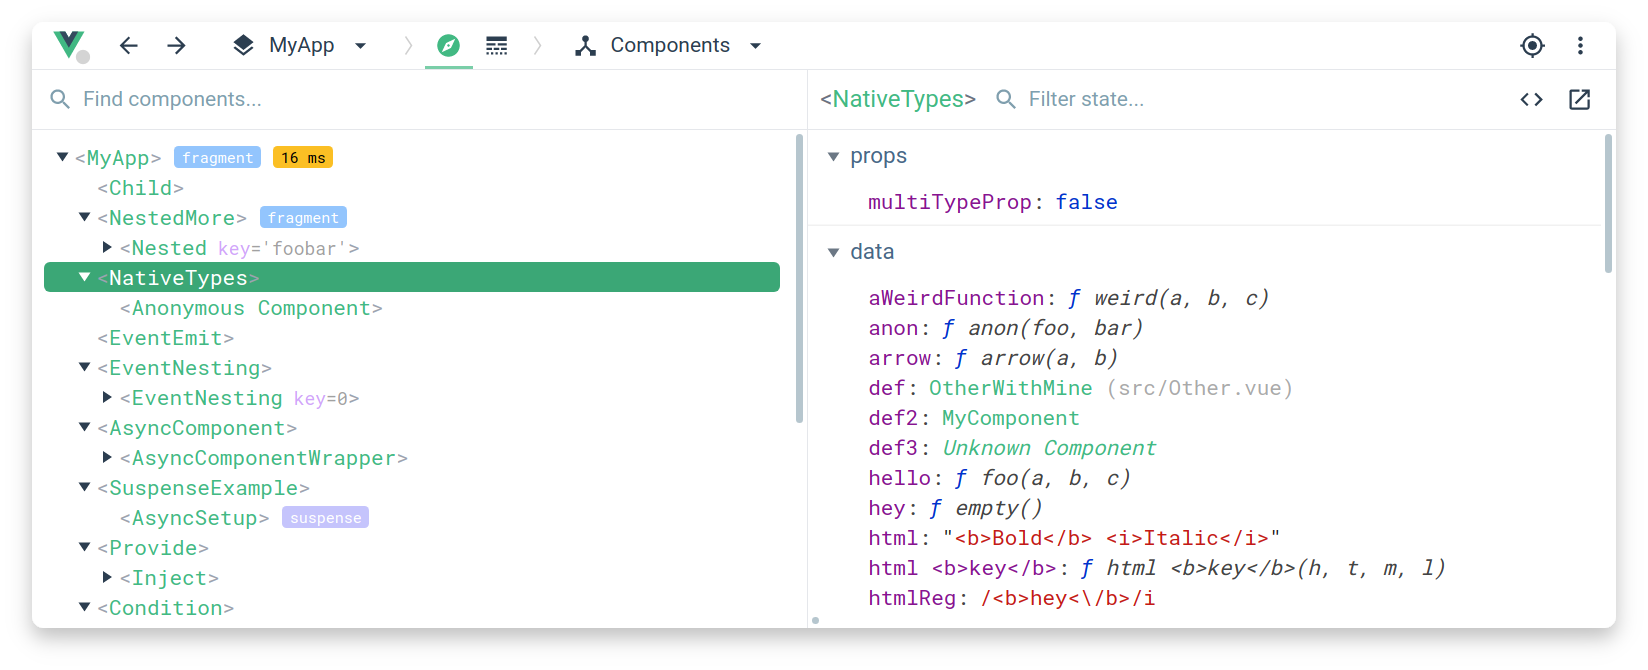
\includegraphics{./img/screenshot-shadow.png} 
\end{center}
    

\columnratio{0.55}
\begin{paracol}{2}
 
\switchcolumn[0]*%%%%%%%
\begin{itemize}
\item
  \href{https://devtools.vuejs.org/}{Documentation}
\item
  \href{https://chrome.google.com/webstore/detail/vuejs-devtools/nhdogjmejiglipccpnnnanhbledajbpd}{Chrome
  Extension}
\item
  \href{https://addons.mozilla.org/en-US/firefox/addon/vue-js-devtools/}{Firefox
  Addon}
\item
  \href{https://microsoftedge.microsoft.com/addons/detail/vuejs-devtools/olofadcdnkkjdfgjcmjaadnlehnnihnl}{Edge
  Extension}
\item
  \href{https://devtools.vuejs.org/guide/installation.html\#standalone}{Standalone
  Electron app}
\end{itemize}
\switchcolumn
\begin{itemize}
\item
  \href{https://devtools.vuejs.org/}{文档}
\item
  \href{https://chrome.google.com/webstore/detail/vuejs-devtools/nhdogjmejiglipccpnnnanhbledajbpd}{Chrome
  扩展商店页}
\item
  \href{https://addons.mozilla.org/en-US/firefox/addon/vue-js-devtools/}{Firefox
  所属插件页}
\item
  \href{https://microsoftedge.microsoft.com/addons/detail/vuejs-devtools/olofadcdnkkjdfgjcmjaadnlehnnihnl}{Edge
  扩展}
\item
  \href{https://devtools.vuejs.org/guide/installation.html\#standalone}{独立的
  Electron 应用所属插件}
\end{itemize}
\end{paracol}

\columnratio{0.55}
\begin{paracol}{2}
 
\switchcolumn[0]*%%%%%%%
\subsection{TypeScript}
\switchcolumn
\subsection{TypeScript}
\switchcolumn[0]*%%%%%%%
Main article:
\href{https://vuejs.org/guide/typescript/overview.html}{Using Vue with
TypeScript}.
\switchcolumn
具体细节请参考章节:\href{https://cn.vuejs.org/guide/typescript/overview.html}{配合
TypeScript 使用 Vue}。
\switchcolumn[0]*%%%%%%%
\begin{itemize}
\item
  \href{https://github.com/johnsoncodehk/volar}{Volar} provides type
  checking for SFCs using
  \texttt{\textless{}script\ lang="ts"\textgreater{}} blocks, including
  template expressions and cross-component props validation.
\item
  Use
  \href{https://github.com/vuejs/language-tools/tree/master/packages/tsc}{\texttt{vue-tsc}}
  for performing the same type checking from the command line, or for
  generating \texttt{d.ts} files for SFCs.
\end{itemize}
\switchcolumn
\begin{itemize}
\item
  \href{https://github.com/johnsoncodehk/volar}{Volar} 插件能够为
  \texttt{\textless{}script\ lang="ts"\textgreater{}}
  块提供类型检查,也能对模板内表达式和组件之间 props
  提供自动补全和类型验证。
\item
  使用
  \href{https://github.com/vuejs/language-tools/tree/master/packages/tsc}{\texttt{vue-tsc}}
  可以在命令行中执行相同的类型检查,通常用来生成单文件组件的
  \texttt{d.ts} 文件。
\end{itemize} 
\switchcolumn[0]*%%%%%%%
\subsection{Testing}
\switchcolumn
\subsection{测试}
\switchcolumn[0]*%%%%%%%
Main article:
\href{https://vuejs.org/guide/scaling-up/testing.html}{Testing Guide}.
\switchcolumn
具体细节请参考章节:\href{https://cn.vuejs.org/guide/scaling-up/testing.html}{测试指南}。
\switchcolumn[0]*%%%%%%%
\begin{itemize}
\item
  \href{https://www.cypress.io/}{Cypress} is recommended for E2E tests.
  It can also be used for component testing for Vue SFCs via the
  \href{https://docs.cypress.io/guides/component-testing/introduction}{Cypress
  Component Test Runner}.
\item
  \href{https://vitest.dev/}{Vitest} is a test runner created by Vue /
  Vite team members that focuses on speed. It is specifically designed
  for Vite-based applications to provide the same instant feedback loop
  for unit / component testing.
\item
  \href{https://jestjs.io/}{Jest} can be made to work with Vite via
  \href{https://github.com/sodatea/vite-jest}{vite-jest}. However, this
  is only recommended if you have existing Jest-based test suites that
  you need to migrate over to a Vite-based setup, as Vitest provides
  similar functionalities with a much more efficient integration.
\end{itemize}
\switchcolumn
\begin{itemize}
\item
  \href{https://www.cypress.io/}{Cypress} 推荐用于 E2E 测试。也可以通过
  \href{https://docs.cypress.io/guides/component-testing/introduction}{Cypress
  组件测试运行器}来给 Vue SFC 作单文件组件测试。
\item
  \href{https://vitest.dev/}{Vitest}
  是一个追求更快运行速度的测试运行器,由 Vue / Vite
  团队成员开发。主要针对基于 Vite
  的应用设计,可以为组件提供即时响应的测试反馈。
\item
  \href{https://jestjs.io/}{Jest} 可以通过
  \href{https://github.com/sodatea/vite-jest}{vite-jest} 配合 Vite
  使用。不过只推荐在你已经有一套基于 Jest 的测试集、且想要迁移到基于
  Vite 的开发配置时使用,因为 Vitest 也能够提供类似的功能,且后者与 Vite
  的集成更方便高效。
\end{itemize}
\switchcolumn[0]*%%%%%%%
\subsection{Linting}
\switchcolumn
\subsection{代码规范}
\switchcolumn[0]*%%%%%%%
The Vue team maintains
\href{https://github.com/vuejs/eslint-plugin-vue}{eslint-plugin-vue}, an
\href{https://eslint.org/}{ESLint} plugin that supports SFC-specific
linting rules.
\switchcolumn
Vue 团队维护着
\href{https://github.com/vuejs/eslint-plugin-vue}{eslint-plugin-vue}
项目,它是一个 \href{https://eslint.org/}{ESLint} 插件,会提供 SFC
相关规则的定义。
\switchcolumn[0]*%%%%%%%
Users previously using Vue CLI may be used to having linters configured
via webpack loaders. However when using a Vite-based build setup, our
general recommendation is:
\switchcolumn
之前使用 Vue CLI 的用户可能习惯于通过 webpack loader
来配置规范检查器。然而,若基于 Vite 构建,我们一般推荐:
\switchcolumn[0]*%%%%%%%
\begin{enumerate}
\item
  \texttt{npm\ install\ -D\ eslint\ eslint-plugin-vue}, then follow
  \texttt{eslint-plugin-vue}'s
  \href{https://eslint.vuejs.org/user-guide/\#usage}{configuration
  guide}.
\item
  Setup ESLint IDE extensions, for example
  \href{https://marketplace.visualstudio.com/items?itemName=dbaeumer.vscode-eslint}{ESLint
  for VSCode}, so you get linter feedback right in your editor during
  development. This also avoids unnecessary linting cost when starting
  the dev server.
\item
  Run ESLint as part of the production build command, so you get full
  linter feedback before shipping to production.
\item
  (Optional) Setup tools like
  \href{https://github.com/okonet/lint-staged}{lint-staged} to
  automatically lint modified files on git commit.
\end{enumerate}
\switchcolumn
\begin{enumerate}
\item
  \texttt{npm\ install\ -D\ eslint\ eslint-plugin-vue},然后遵照
  \texttt{eslint-plugin-vue}
  的\href{https://eslint.vuejs.org/user-guide/\#usage}{指引}进行配置。
\item
  启用 ESLint IDE 插件,比如
  \href{https://marketplace.visualstudio.com/items?itemName=dbaeumer.vscode-eslint}{ESLint
  for
  VSCode},然后你就可以在开发时获得规范检查器的反馈。这同时也避免了启动开发服务器时不必要的规范检查。
\item
  将 ESLint
  格式检查作为一个生产构建的步骤,保证你可以在最终打包时获得完整的规范检查反馈。
\item
  (可选) 启用类似
  \href{https://github.com/okonet/lint-staged}{lint-staged} 一类的工具在
  git commit 提交时自动执行规范检查。
\end{enumerate}
\end{paracol}

\columnratio{0.55}
\begin{paracol}{2}
 
\switchcolumn[0]*%%%%%%%
\subsection{Formatting}
\switchcolumn
\subsection{格式化}
\switchcolumn[0]*%%%%%%%
\begin{itemize}
\item
  The \href{https://github.com/johnsoncodehk/volar}{Volar} VSCode
  extension provides formatting for Vue SFCs out of the box.
\item
  Alternatively, \href{https://prettier.io/}{Prettier} provides built-in
  Vue SFC formatting support.
\end{itemize}
\switchcolumn
\begin{itemize}
\item
  \href{https://github.com/johnsoncodehk/volar}{Volar} VSCode 插件为 Vue
  SFC 提供了开箱即用的格式化功能。
\item
  除此之外,\href{https://prettier.io/}{Prettier} 也提供了内置的 Vue SFC
  格式化支持。
\end{itemize}
\switchcolumn[0]*%%%%%%%
\subsection{SFC Custom Block Integrations}
\switchcolumn
\subsection{SFC 自定义块集成}
\switchcolumn[0]*%%%%%%%
Custom blocks are compiled into imports to the same Vue file with
different request queries. It is up to the underlying build tool to
handle these import requests.
\switchcolumn
自定义块被编译成导入到同一 Vue
文件的不同请求查询。这取决于底层构建工具如何处理这类导入请求。
\switchcolumn[0]*%%%%%%%
\begin{itemize}
\item
  If using Vite, a custom Vite plugin should be used to transform
  matched custom blocks into executable JavaScript.
  \href{https://github.com/vitejs/vite-plugin-vue/tree/main/packages/plugin-vue\#example-for-transforming-custom-blocks}{Example}
\item
  If using Vue CLI or plain webpack, a webpack loader should be
  configured to transform the matched blocks.
  \href{https://vue-loader.vuejs.org/guide/custom-blocks.html}{Example}
\end{itemize}
\switchcolumn
\begin{itemize}
\item
  如果使用 Vite,需使用一个自定义 Vite 插件将自定义块转换为可执行的
  JavaScript
  代码。\href{https://github.com/vitejs/vite-plugin-vue/tree/main/packages/plugin-vue\#example-for-transforming-custom-blocks}{示例}。
\item
  如果使用 Vue CLI 或只是 webpack,需要使用一个 loader
  来配置如何转换匹配到的自定义块。\href{https://vue-loader.vuejs.org/zh/guide/custom-blocks.html}{示例}。
\end{itemize}
\switchcolumn[0]*%%%%%%%
\subsection{Lower-Level Packages}
\switchcolumn
\subsection{底层库}
\switchcolumn[0]*%%%%%%%
\subsubsection{@vue/compiler-sfc}
\switchcolumn
\subsubsection{@vue/compiler-sfc}
\switchcolumn[0]*%%%%%%%
\begin{itemize}
\item
  \href{https://github.com/vuejs/core/tree/main/packages/compiler-sfc}{Docs}
\end{itemize}
\switchcolumn
\begin{itemize}
\item
  \href{https://github.com/vuejs/core/tree/main/packages/compiler-sfc}{文档}
\end{itemize}
\switchcolumn[0]*%%%%%%%
This package is part of the Vue core monorepo and is always published
with the same version as the main \texttt{vue} package. It is included
as a dependency of the main \texttt{vue} package and proxied under
\texttt{vue/compiler-sfc} so you don't need to install it individually.
\switchcolumn
这个包是 Vue 核心 monorepo 的一部分,并始终和 \texttt{vue}
主包版本号保持一致。它已经成为 \texttt{vue} 主包的一个依赖并代理到了
\texttt{vue/compiler-sfc} 目录下,因此你无需单独安装它。
\switchcolumn[0]*%%%%%%%
The package itself provides lower-level utilities for processing Vue
SFCs and is only meant for tooling authors that need to support Vue SFCs
in custom tools.
\switchcolumn
这个包本身提供了处理 Vue SFC 的底层的功能,并只适用于需要支持 Vue SFC
相关工具链的开发者。
\switchcolumn[0]*%%%%%%%
\begin{vueQuote}{TIP}
Always prefer using this package via the \texttt{vue/compiler-sfc} deep
import since this ensures its version is in sync with the Vue runtime.
\end{vueQuote} 
\switchcolumn
\begin{vueQuote}{TIP}
请始终选择通过 \texttt{vue/compiler-sfc}
的深度导入来使用这个包,因为这样可以确保其与 Vue 运行时版本同步。
\end{vueQuote} 
\end{paracol}

\columnratio{0.55}
\begin{paracol}{2}
 
\switchcolumn[0]*%%%%%%%
\subsubsection{@vitejs/plugin-vue}
\switchcolumn
\subsubsection{@vitejs/plugin-vue}
\switchcolumn[0]*%%%%%%%
\begin{itemize}
\item
  \href{https://github.com/vitejs/vite-plugin-vue/tree/main/packages/plugin-vue}{Docs}
\end{itemize}
\switchcolumn
\begin{itemize}
\item
  \href{https://github.com/vitejs/vite-plugin-vue/tree/main/packages/plugin-vue}{文档}
\end{itemize}
\switchcolumn[0]*%%%%%%%
Official plugin that provides Vue SFC support in Vite.
\switchcolumn
为 Vite 提供 Vue SFC 支持的官方插件。
\switchcolumn[0]*%%%%%%%
\subsubsection{vue-loader}
\switchcolumn
\subsubsection{vue-loader}
\switchcolumn[0]*%%%%%%%
\begin{itemize}
\item
  \href{https://vue-loader.vuejs.org/}{Docs}
\end{itemize}
\switchcolumn
\begin{itemize}
\item
  \href{https://vue-loader.vuejs.org/zh/}{文档}
\end{itemize}
\switchcolumn[0]*%%%%%%%
The official loader that provides Vue SFC support in webpack. If you are
using Vue CLI, also see
\href{https://cli.vuejs.org/guide/webpack.html\#modifying-options-of-a-loader}{docs
on modifying \texttt{vue-loader} options in Vue CLI}.
\switchcolumn
为 webpack 提供 Vue SFC 支持的官方 loader。如果你正在使用 Vue
CLI,也可以看看\href{https://cli.vuejs.org/zh/guide/webpack.html\#修改-loader-选项}{如何在
Vue CLI 中更改 \texttt{vue-loader} 选项的文档}。
\switchcolumn[0]*%%%%%%%
\subsection{Other Online Playgrounds}
\switchcolumn
\subsection{其他在线演练场}
\switchcolumn[0]*%%%%%%%
\begin{itemize}
\item
  \href{https://play.vueuse.org/}{VueUse Playground}
\item
  \href{https://replit.com/@templates/VueJS-with-Vite}{Vue + Vite on
  Repl.it}
\item
  \href{https://codesandbox.io/s/vue-3}{Vue on CodeSandbox}
\item
  \href{https://codepen.io/pen/editor/vue}{Vue on Codepen}
\item
  \href{https://components.studio/create/vue3}{Vue on Components.studio}
\item
  \href{https://webcomponents.dev/create/cevue}{Vue on
  WebComponents.dev}
\end{itemize}
\switchcolumn
\begin{itemize}
\item
  \href{https://play.vueuse.org/}{VueUse Playground}
\item
  \href{https://replit.com/@templates/VueJS-with-Vite}{Vue + Vite on
  Repl.it}
\item
  \href{https://codesandbox.io/s/vue-3}{Vue on CodeSandbox}
\item
  \href{https://codepen.io/pen/editor/vue}{Vue on Codepen}
\item
  \href{https://components.studio/create/vue3}{Vue on Components.studio}
\item
  \href{https://webcomponents.dev/create/cevue}{Vue on
  WebComponents.dev}
\end{itemize}
\end{paracol}
 